\documentclass[sigconf]{acmart}

\usepackage{soul}
\usepackage{xcolor}
\newcommand{\pending}[1]{\hl{#1}} % marca texto como pendente
\sethlcolor{yellow} % cor do highlight
%%
%% \BibTeX command to typeset BibTeX logo in the docs
\AtBeginDocument{%
  \providecommand\BibTeX{{%
    Bib\TeX}}}

%% Rights management information.  This information is sent to you
%% when you complete the rights form.  These commands have SAMPLE
%% values in them; it is your responsibility as an author to replace
%% the commands and values with those provided to you when you
%% complete the rights form.
\setcopyright{acmlicensed}
\copyrightyear{2018}
\acmYear{2018}
\acmDOI{XXXXXXX.XXXXXXX}
%% These commands are for a PROCEEDINGS abstract or paper.
\acmConference[Conference acronym 'XX]{Make sure to enter the correct
  conference title from your rights confirmation email}{June 03--05,
  2018}{Woodstock, NY}
%%
%%  Uncomment \acmBooktitle if the title of the proceedings is different
%%  from ``Proceedings of ...''!
%%
%%\acmBooktitle{Woodstock '18: ACM Symposium on Neural Gaze Detection,
%%  June 03--05, 2018, Woodstock, NY}
\acmISBN{978-1-4503-XXXX-X/2018/06}

%%
%% end of the preamble, start of the body of the document source.
\begin{document}

%%
%% The "title" command has an optional parameter,
%% allowing the author to define a "short title" to be used in page headers.
\title{The nome of the Title Is Hope}

%%
%% The "author" command and its associated commands are used to define
%% the authors and their affiliations.
%% Of note is the shared affiliation of the first two authors, and the
%% "authornote" and "authornotemark" commands
%% used to denote shared contribution to the research.
\author{Robson Gonçalves}
%%\authornote{Both authors contributed equally to this research.}
\email{robson.o.goncalves@posgrad.ufsc.br}
\orcid{1234-5678-9012}
%%\author{G.K.M. Tobin}
%%\authornotemark[1]
%%\email{webmaster@marysville-ohio.com}
\affiliation{%
  \institution{University Federal of Santa Catarina}
  \city{Florianopolis}
  \state{SC}
  \country{Brazil}
}

\author{Carina F Dorneles}
\email{carina.dorneles@ufsc.br}
\affiliation{%
  \institution{University Federal of Santa Catarina}
  \city{Florianopolis}
  \country{Brazil}}

\author{XXX}
\email{xxx@ufsc.br}
\affiliation{%
  \institution{University Federal of Santa Catarina}
  \city{Florianopolis}
  \country{Brazil}
}

%%
%% By default, the full list of authors will be used in the page
%% headers. Often, this list is too long, and will overlap
%% other information printed in the page headers. This command allows
%% the author to define a more concise list
%% of authors' names for this purpose.
\renewcommand{\shortauthors}{Gonçalves et al.}

%%
%% The abstract is a short summary of the work to be presented in the
%% article.
\begin{abstract}
  A clear and well-documented \LaTeX\ document is presented as an
  article formatted for publication by ACM in a conference proceedings
  or journal publication. Based on the ``acmart'' document class, this
  article presents and explains many of the common variations, as well
  as many of the formatting elements an author may use in the
  preparation of the documentation of their work.
\end{abstract}


%%
%% Keywords. The author(s) should pick words that accurately describe
%% the work being presented. Separate the keywords with commas.
\keywords{Do, Not, Use, This, Code, Put, the, Correct, Terms, for,
  Your, Paper}
%% A "teaser" image appears between the author and affiliation
%% information and the body of the document, and typically spans the
%% page.
% \begin{teaserfigure}
%   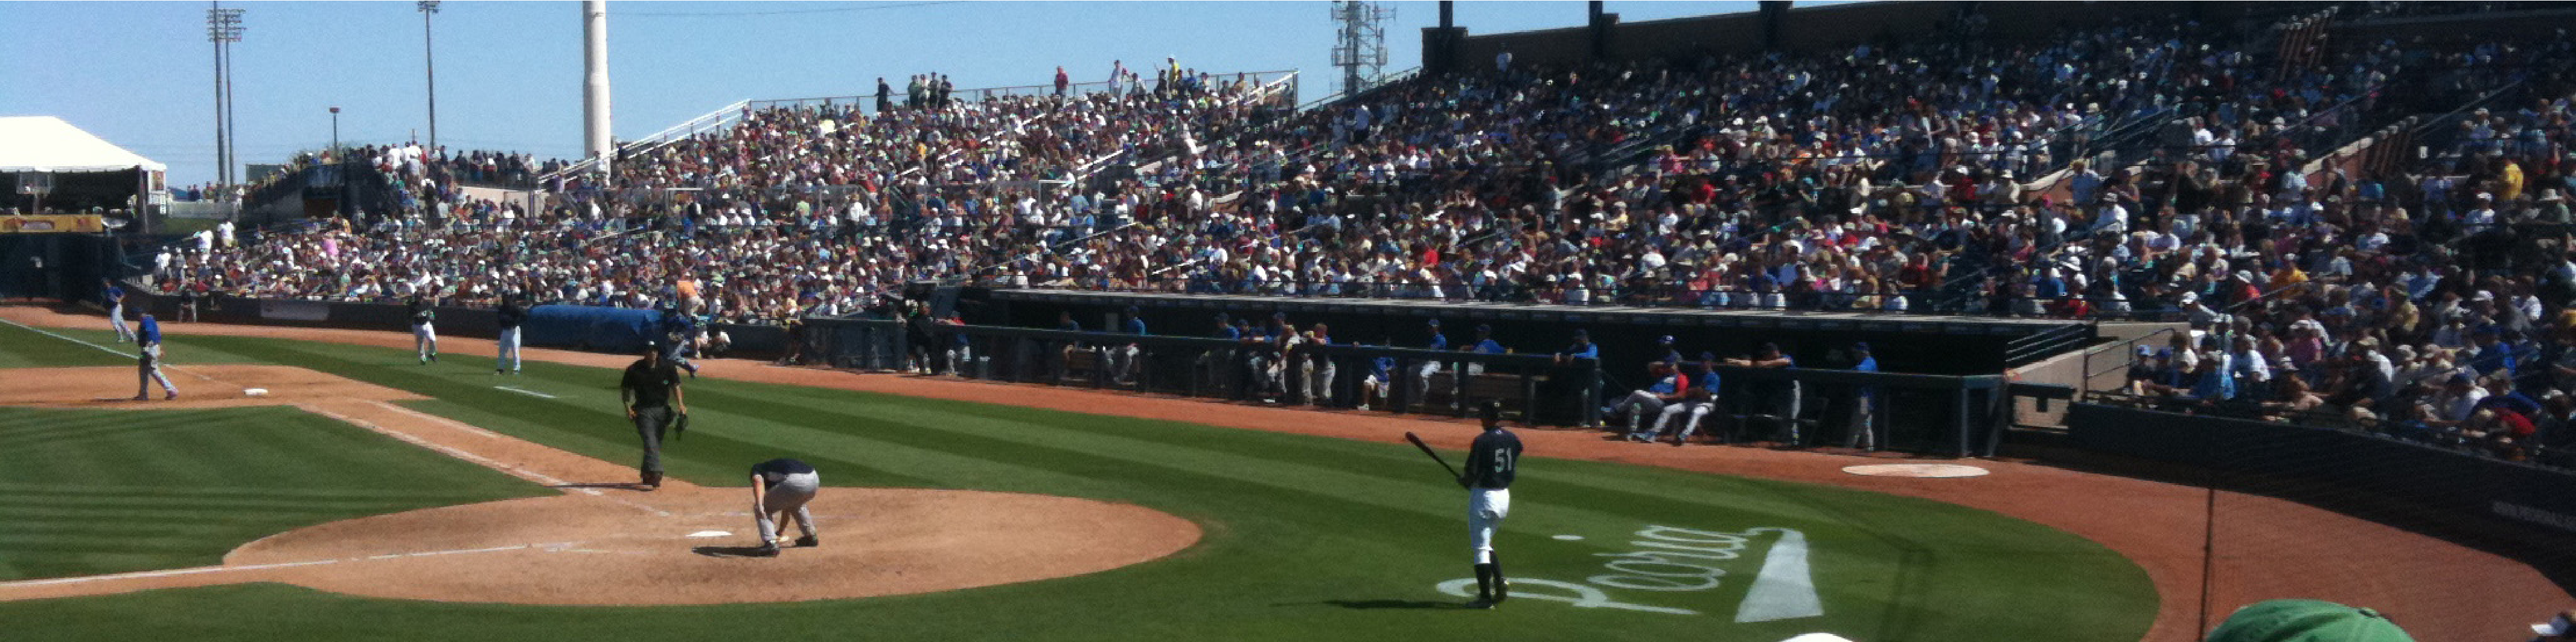
\includegraphics[width=\textwidth]{sampleteaser}
%   \caption{Seattle Mariners at Spring Training, 2010.}
%   \Description{Enjoying the baseball game from the third-base
%   seats. Ichiro Suzuki preparing to bat.}
%   \label{fig:teaser}
% \end{teaserfigure}

\received{20 February 2007}
\received[revised]{12 March 2009}
\received[accepted]{5 June 2009}

%%
%% This command processes the author and affiliation and title
%% information and builds the first part of the formatted document.
\maketitle

\section{Introduction}
%Paragrafo 1: contexto do artigo.
LLMs (Large Language Models) have been widely used for information extraction from documents.
Information Extraction (IE) is a crucial domain in natural
language processing (NLP) that converts plain text into
structured knowledge (e.g., entities, relations, and events), and
serves as a foundational requirement for a wide range of
downstream tasks, such as knowledge graph construction,
knowledge reasoning, and question answering. Typical
IE tasks consist of Named Entity Recognition (NER), Relation
Extraction (RE) and Event Extraction (EE)\cite{Xu2024}.
The development history of information extraction technology has three methods:
the method based on rules and dictionaries, the method based on statistical machine learning,
and the method based on deep learning \cite{Yang2022}.
% falta os tipos de extração.

%Paragrafo 2: problema. 
Due to size and complexity of such data, the IE is a tedious
task because it involves the format sensitive approaches whose
effectiveness fluctuates severely with the slight change in the
format of the documents. That is why, no single win-win
scheme has been introduced that can handle all formats at the
same time \cite{Rahman2022}.

Paragrafo 3: trabalhos relacionados.

Paragrafo 4: contribuições do artigo. descrever o uso do modelo Hierarcical Reasioning Model para extração de informações de documentos.
Este artigo trata uma proposta de uso do modelo Hierarcical Reasioning Model para extração de informações de documentos. 
E as contribuições são: 
1.utilizar um cenario de extração de informações de documentos utilizando HRM. 
2.apresentar um dataset de dados específico para treinar o modelo HRM. 
3.avaliar o desempenho deste modelo em relação aos modelos tradicionais.

um modelo de extração de informações de documentos que utiliza o modelo Hierarcical Reasioning Model e avaliar o desempenho do modelo em relação aos modelos existentes.
Paragrafo 5: estrutura do artigo.

\section{Related Work}
Trabalhos relacionados.


\pending{
  Em Zhou2022, oferece uma revisão abrangente sobre técnicas de Extração de Informação (IE) baseadas em aprendizado profundo (Deep Learning, DL), destacando a transição de métodos tradicionais — baseados em regras e estatísticas — para abordagens modernas fundamentadas em redes neurais. A análise mostra que, em tarefas como Reconhecimento de Entidades Nomeadas (NER), Extração de Relações (RE) e Extração de Eventos (EE), os métodos de DL, especialmente arquiteturas como CNNs, RNNs, LSTMs, GNNs e modelos híbridos, superaram os métodos anteriores ao reduzir a dependência de engenharia manual de atributos e melhorar a capacidade de generalização. 
  Em particular, observa-se que modelos conjuntos (joint extraction) são mais eficientes do que o paradigma pipeline, por resolverem problemas de propagação de erro e aproveitarem melhor as dependências linguísticas entre entidades e relações. Além disso, o trabalho enfatiza que técnicas recentes de supervisão distante e incorporação de conhecimento (knowledge embedding) têm ampliado a robustez dos modelos, ainda que desafios como ruído em dados anotados automaticamente e a dificuldade de lidar com relações sobrepostas permaneçam abertos  
}\cite{Zhou2022}


\section{Experimental Evaluation}
Metodologia do artigo.

Dataset utilizado com tamanho , link, dominio.

Ambiente: configuracoes do ambiente, variaveis, espec da maquina

passo a passo: foi feito isso, feito aquilo, etc

metricas: escala, precisao, tempo, revocação

\section{Results and Discussion}
Resultados do artigo.

Graficos das metricas

Discussões sobre graficos, resultados, metricas


\section{Conclusion}
Conclusão do artigo.

\pending{explicar motivação aqui}
% \todo[inline]{mover esta seção para Related Work}

Breve resumo sem novidades. nao pode deixar itens que nao foram discutidos no artigo. 
trabalhos futuros o que pode ser feito alem do que foi apresentado.



%%
%% The acknowledgments section is defined using the "acks" environment
%% (and NOT an unnumbered section). This ensures the proper
%% identification of the section in the article metadata, and the
%% consistent spelling of the heading.
\begin{acks}
To Robert, for the bagels and explaining CMYK and color spaces.
\end{acks}

%%
%% The next two lines define the bibliography style to be used, and
%% the bibliography file.
\bibliographystyle{ACM-Reference-Format}
\bibliography{sample-base}
\end{document}
\endinput
%%
%% End of file `sample-sigconf.tex'.
